\documentclass[12pt,a4paper]{article}

\usepackage[a4paper,margin=1in]{geometry}
\usepackage[final]{graphicx}
\graphicspath{{images/}{./}{experiment_7/images/}}
\usepackage{booktabs}
\usepackage{amsmath,amssymb}
\usepackage{float}
\usepackage{hyperref}
\usepackage{xcolor}
\usepackage{listings}
\usepackage{enumitem}
\usepackage{fancyhdr}
\usepackage{longtable}
\usepackage{array}
\usepackage{multirow}
\usepackage{tabularx}

\hypersetup{colorlinks=true,linkcolor=blue,urlcolor=blue}

\pagestyle{fancy}
\fancyhf{}
\lhead{ICS1512}
\rhead{Machine Learning Algorithms Laboratory}
\cfoot{\thepage}

\lstset{
language=Python,
basicstyle=\ttfamily\small,
numbers=left,
frame=single,
breaklines=true,
showstringspaces=false,
keywordstyle=\color{blue},
commentstyle=\color{gray},
stringstyle=\color{orange}
}

\begin{document}

% =====================================================================
% EXPERIMENT 7: DIMENSIONALITY REDUCTION AND MODEL EVALUATION (WITH AND WITHOUT PCA)
% =====================================================================

\begin{tabular}{|p{4cm}|p{11cm}|}
\hline
Experiment No. & 7 \\ \hline
Experiment Title & Dimensionality Reduction using Principal Component Analysis (PCA) and Comprehensive Model Evaluation \textsuperscript{\href{https://github.com/arivuchezhiyan/Machine_Learning/tree/main/experiment_7}{7}} \\ \hline
Student Name & Arivuchezhiyan E \\ \hline
Register Number & 3122247001006 \\ \hline
Faculty & Dr. Poreddy Ajay Kumar Reddy \\ \hline
Submission Date & 23/07/2026 \\ \hline
\end{tabular}

\vspace{0.5cm}

\section{Objective}
State the objective of the experiment:

In this laboratory experiment, my main objective was to conduct a comprehensive empirical study on the impact of dimensionality reduction via Principal Component Analysis (PCA) across ten diverse supervised machine learning classifiers. Using the Wisconsin Diagnostic Breast Cancer (WDBC) benchmark dataset, I systematically trained, tuned, cross-validated and tested ten classification algorithms under two comparative settings:
\begin{enumerate}
\item \textbf{Without PCA}: Training and validating models on the original 30-dimensional standardized feature space.
\item \textbf{With PCA}: Training and validating models on an orthogonally transformed, lower-dimensional subspace capturing 95\% of total dataset variance.
\end{enumerate}

Specific investigation objectives included:
\begin{itemize}
\item Performing eigendecomposition of the sample covariance matrix and plotting scree curves to determine optimal intrinsic dimensionality.
\item Evaluating ten distinct classification algorithms: Support Vector Machine (SVM), Gaussian Naive Bayes, k-Nearest Neighbors (KNN), Logistic Regression, Decision Tree, Random Forest, AdaBoost, Gradient Boosting, XGBoost and Stacking.
\item Executing systematic hyperparameter grid searches under 5-fold Stratified Cross-Validation for both No-PCA and With-PCA feature representations.
\item Analyzing variance reduction, overfitting mitigation, decision boundary deformation and computational efficiency trade-offs caused by orthogonal subspace projection.
\item Assessing final diagnostic discrimination through confusion matrix contingency breakdowns, multi-model ROC-AUC curves and fold-wise stability metrics.
\end{itemize}

\section{Problem Statement}
Describe the problem input output and objective:

High-dimensional medical cytology datasets frequently contain severe multicollinearity and redundant measurements across morphometric cell attributes. While abundant features provide diagnostic signal, excessive dimensionality can induce the curse of dimensionality, increase model variance, inflate computational training cost and degrade distance-based estimators.

The machine learning task is formulated as follows:
\begin{itemize}
\item \textbf{Input}: A standardized continuous feature vector $x \in \mathbb{R}^{30}$ containing thirty nuclear morphometric measurements (radii, perimeters, areas, textures, smoothness, concavities and symmetry metrics) or its PCA projection $z \in \mathbb{R}^{k}$ where $k \ll 30$.
\item \textbf{Output}: Binary target classification label $y \in \{0, 1\}$ denoting tissue condition where 0 represents a Malignant mass and 1 represents a Benign mass.
\item \textbf{Objective}: Formulate the mathematical foundation of PCA, perform feature standardization, compute the cumulative variance spectrum to choose optimal components $k$, define hyperparameter grids for ten classifiers, evaluate fold-by-fold cross-validation performance under No-PCA and With-PCA modes, evaluate generalization on an independent test partition and analyze which model families benefit most from dimensionality reduction.
\end{itemize}

\section{Dataset Description}

The experiment evaluates the Wisconsin Diagnostic Breast Cancer (WDBC) dataset obtained from the UCI Machine Learning Repository.

\begin{longtable}{|p{6cm}|p{8cm}|}
\hline
\textbf{Dataset Attribute} & \textbf{Specification} \\ \hline
Dataset Name & Wisconsin Diagnostic Breast Cancer (WDBC) \\ \hline
Data Source & \texttt{sklearn.datasets.load\_breast\_cancer} / wdbc.csv \\ \hline
Application Domain & Clinical Cytology / Medical Diagnostic Screening \\ \hline
Total Sample Count & 569 patient instances \\ \hline
Original Feature Count & 30 continuous real-valued morphometric descriptors \\ \hline
Reduced Feature Count (PCA) & 10 principal components ($\ge 95\%$ variance explained) \\ \hline
Target Variable & \texttt{target} (0: Malignant [212 samples], 1: Benign [357 samples]) \\ \hline
Class Distribution Ratio & 62.74\% Benign / 37.26\% Malignant \\ \hline
Missing Values & 0 missing values across all 30 attributes \\ \hline
Train-Test Split & 80\% Training (455 samples) / 20\% Testing (114 samples) \\ \hline
Partitioning Strategy & Stratified random sampling (random\_state = 42) \\ \hline
\end{longtable}

\subsection*{Detailed Feature Attribute Breakdown}
Thirty continuous attributes describe nuclear morphology derived from digitized fine needle aspiration specimens and organized into three statistical subsets of ten basic physical dimensions:
\begin{itemize}
\item \textbf{Mean Descriptors (10 features)}: \texttt{mean radius}, \texttt{mean texture}, \texttt{mean perimeter}, \texttt{mean area}, \texttt{mean smoothness}, \texttt{mean compactness}, \texttt{mean concavity}, \texttt{mean concave points}, \texttt{mean symmetry} and \texttt{mean fractal dimension}.
\item \textbf{Standard Error Descriptors (10 features)}: \texttt{radius error}, \texttt{texture error}, \texttt{perimeter error}, \texttt{area error}, \texttt{smoothness error}, \texttt{compactness error}, \texttt{concavity error}, \texttt{concave points error}, \texttt{symmetry error} and \texttt{fractal dimension error}.
\item \textbf{Worst Descriptors (10 features)}: \texttt{worst radius}, \texttt{worst texture}, \texttt{worst perimeter}, \texttt{worst area}, \texttt{worst smoothness}, \texttt{worst compactness}, \texttt{worst concavity}, \texttt{worst concave points}, \texttt{worst symmetry} and \texttt{worst fractal dimension}.
\end{itemize}

\section{Mathematical Foundation of Principal Component Analysis (PCA)}

Principal Component Analysis is an unsupervised linear transformation technique that identifies orthogonal axes (principal components) maximizing the variance of projected data points while minimizing reconstruction error.

\subsection{Standardization and Covariance Formulation}
Given a data matrix $X \in \mathbb{R}^{N \times p}$ with $N = 455$ training samples and $p = 30$ features, features are first standardized to zero empirical mean and unit empirical variance:
\begin{equation}
z_{ij} = \frac{x_{ij} - \mu_j}{\sigma_j}, \quad \mu_j = \frac{1}{N}\sum_{i=1}^N x_{ij}, \quad \sigma_j^2 = \frac{1}{N}\sum_{i=1}^N (x_{ij} - \mu_j)^2
\end{equation}
The sample covariance matrix $\Sigma \in \mathbb{R}^{p \times p}$ of standardized matrix $Z$ is computed as:
\begin{equation}
\Sigma = \frac{1}{N} Z^T Z
\end{equation}

\subsection{Variance Maximization and Eigendecomposition}
We seek a unit projection vector $v_1 \in \mathbb{R}^p$ ($v_1^T v_1 = 1$) such that the variance of projected coordinates $u_1 = Z v_1$ is maximized:
\begin{equation}
\max_{v_1} \text{Var}(Z v_1) = \max_{v_1} \frac{1}{N} (Z v_1)^T (Z v_1) = \max_{v_1} v_1^T \Sigma v_1 \quad \text{subject to } v_1^T v_1 = 1
\end{equation}
Formulating the Lagrangian with multiplier $\lambda_1$:
\begin{equation}
\mathcal{L}(v_1, \lambda_1) = v_1^T \Sigma v_1 - \lambda_1 (v_1^T v_1 - 1)
\end{equation}
Setting the gradient with respect to $v_1$ to zero yields the fundamental eigenvalue equation:
\begin{equation}
\nabla_{v_1} \mathcal{L} = 2 \Sigma v_1 - 2 \lambda_1 v_1 = 0 \implies \Sigma v_1 = \lambda_1 v_1
\end{equation}
Thus the optimal projection directions correspond to the eigenvectors of $\Sigma$ and the variance along eigenvector $v_j$ is given by eigenvalue $\lambda_j$.

\subsection{Subspace Selection and Explained Variance Ratio}
Sorting the eigenvalues in descending order $\lambda_1 \ge \lambda_2 \ge \dots \ge \lambda_p \ge 0$, the proportion of variance explained by component $j$ is:
\begin{equation}
\text{Explained Variance Ratio}(j) = \frac{\lambda_j}{\sum_{i=1}^p \lambda_i}
\end{equation}
The cumulative explained variance for a $k$-dimensional subspace is:
\begin{equation}
\text{Cumulative Variance}(k) = \frac{\sum_{j=1}^k \lambda_j}{\sum_{i=1}^p \lambda_i}
\end{equation}
Choosing the transformation matrix $W_k = [v_1, v_2, \dots, v_k] \in \mathbb{R}^{p \times k}$, any query sample $x \in \mathbb{R}^p$ is projected into reduced coordinates:
\begin{equation}
z_{\text{reduced}} = W_k^T (x - \mu) \in \mathbb{R}^k
\end{equation}

\section{PCA Variance Analysis and Dimensionality Selection}

Evaluating the cumulative variance spectrum on the WDBC training set indicated that the original 30 correlated features compress into a compact orthogonal subspace:
\begin{itemize}
\item The first principal component (PC1) accounts for **44.27\%** of total dataset variance.
\item The second principal component (PC2) explains **18.97\%** of variance (cumulative 63.24\%).
\item The top six components capture **88.76\%** of variance.
\item Exactly **$k = 10$ principal components** are required to exceed the 95\% cumulative variance threshold, capturing **95.27\%** of total variance while eliminating 20 redundant dimensions (66.7\% reduction in feature space dimensionality).
\end{itemize}

\begin{table}[H]
\centering
\begin{tabular}{|p{3cm}|p{3.5cm}|p{3.5cm}|p{4.5cm}|}
\hline
\textbf{Setting} & \textbf{Chosen Components / Variance Target} & \textbf{Explained Variance (\%)} & \textbf{Justification} \\ \hline
\textbf{No-PCA} & 30 Features & 100.00\% & Full original feature representation preserving raw morphometry. \\ \hline
\textbf{With-PCA} & $k = 10$ Components (Target: 95\%) & \textbf{95.27\%} & Captures over 95\% intrinsic variance, decorrelates features and discards noise dimensions. \\ \hline
\end{tabular}
\caption{Table 1: PCA Variance Explained Summary and Dimensionality Justification}
\label{tab:exp7_pca_summary}
\end{table}

\begin{figure}[H]
\centering
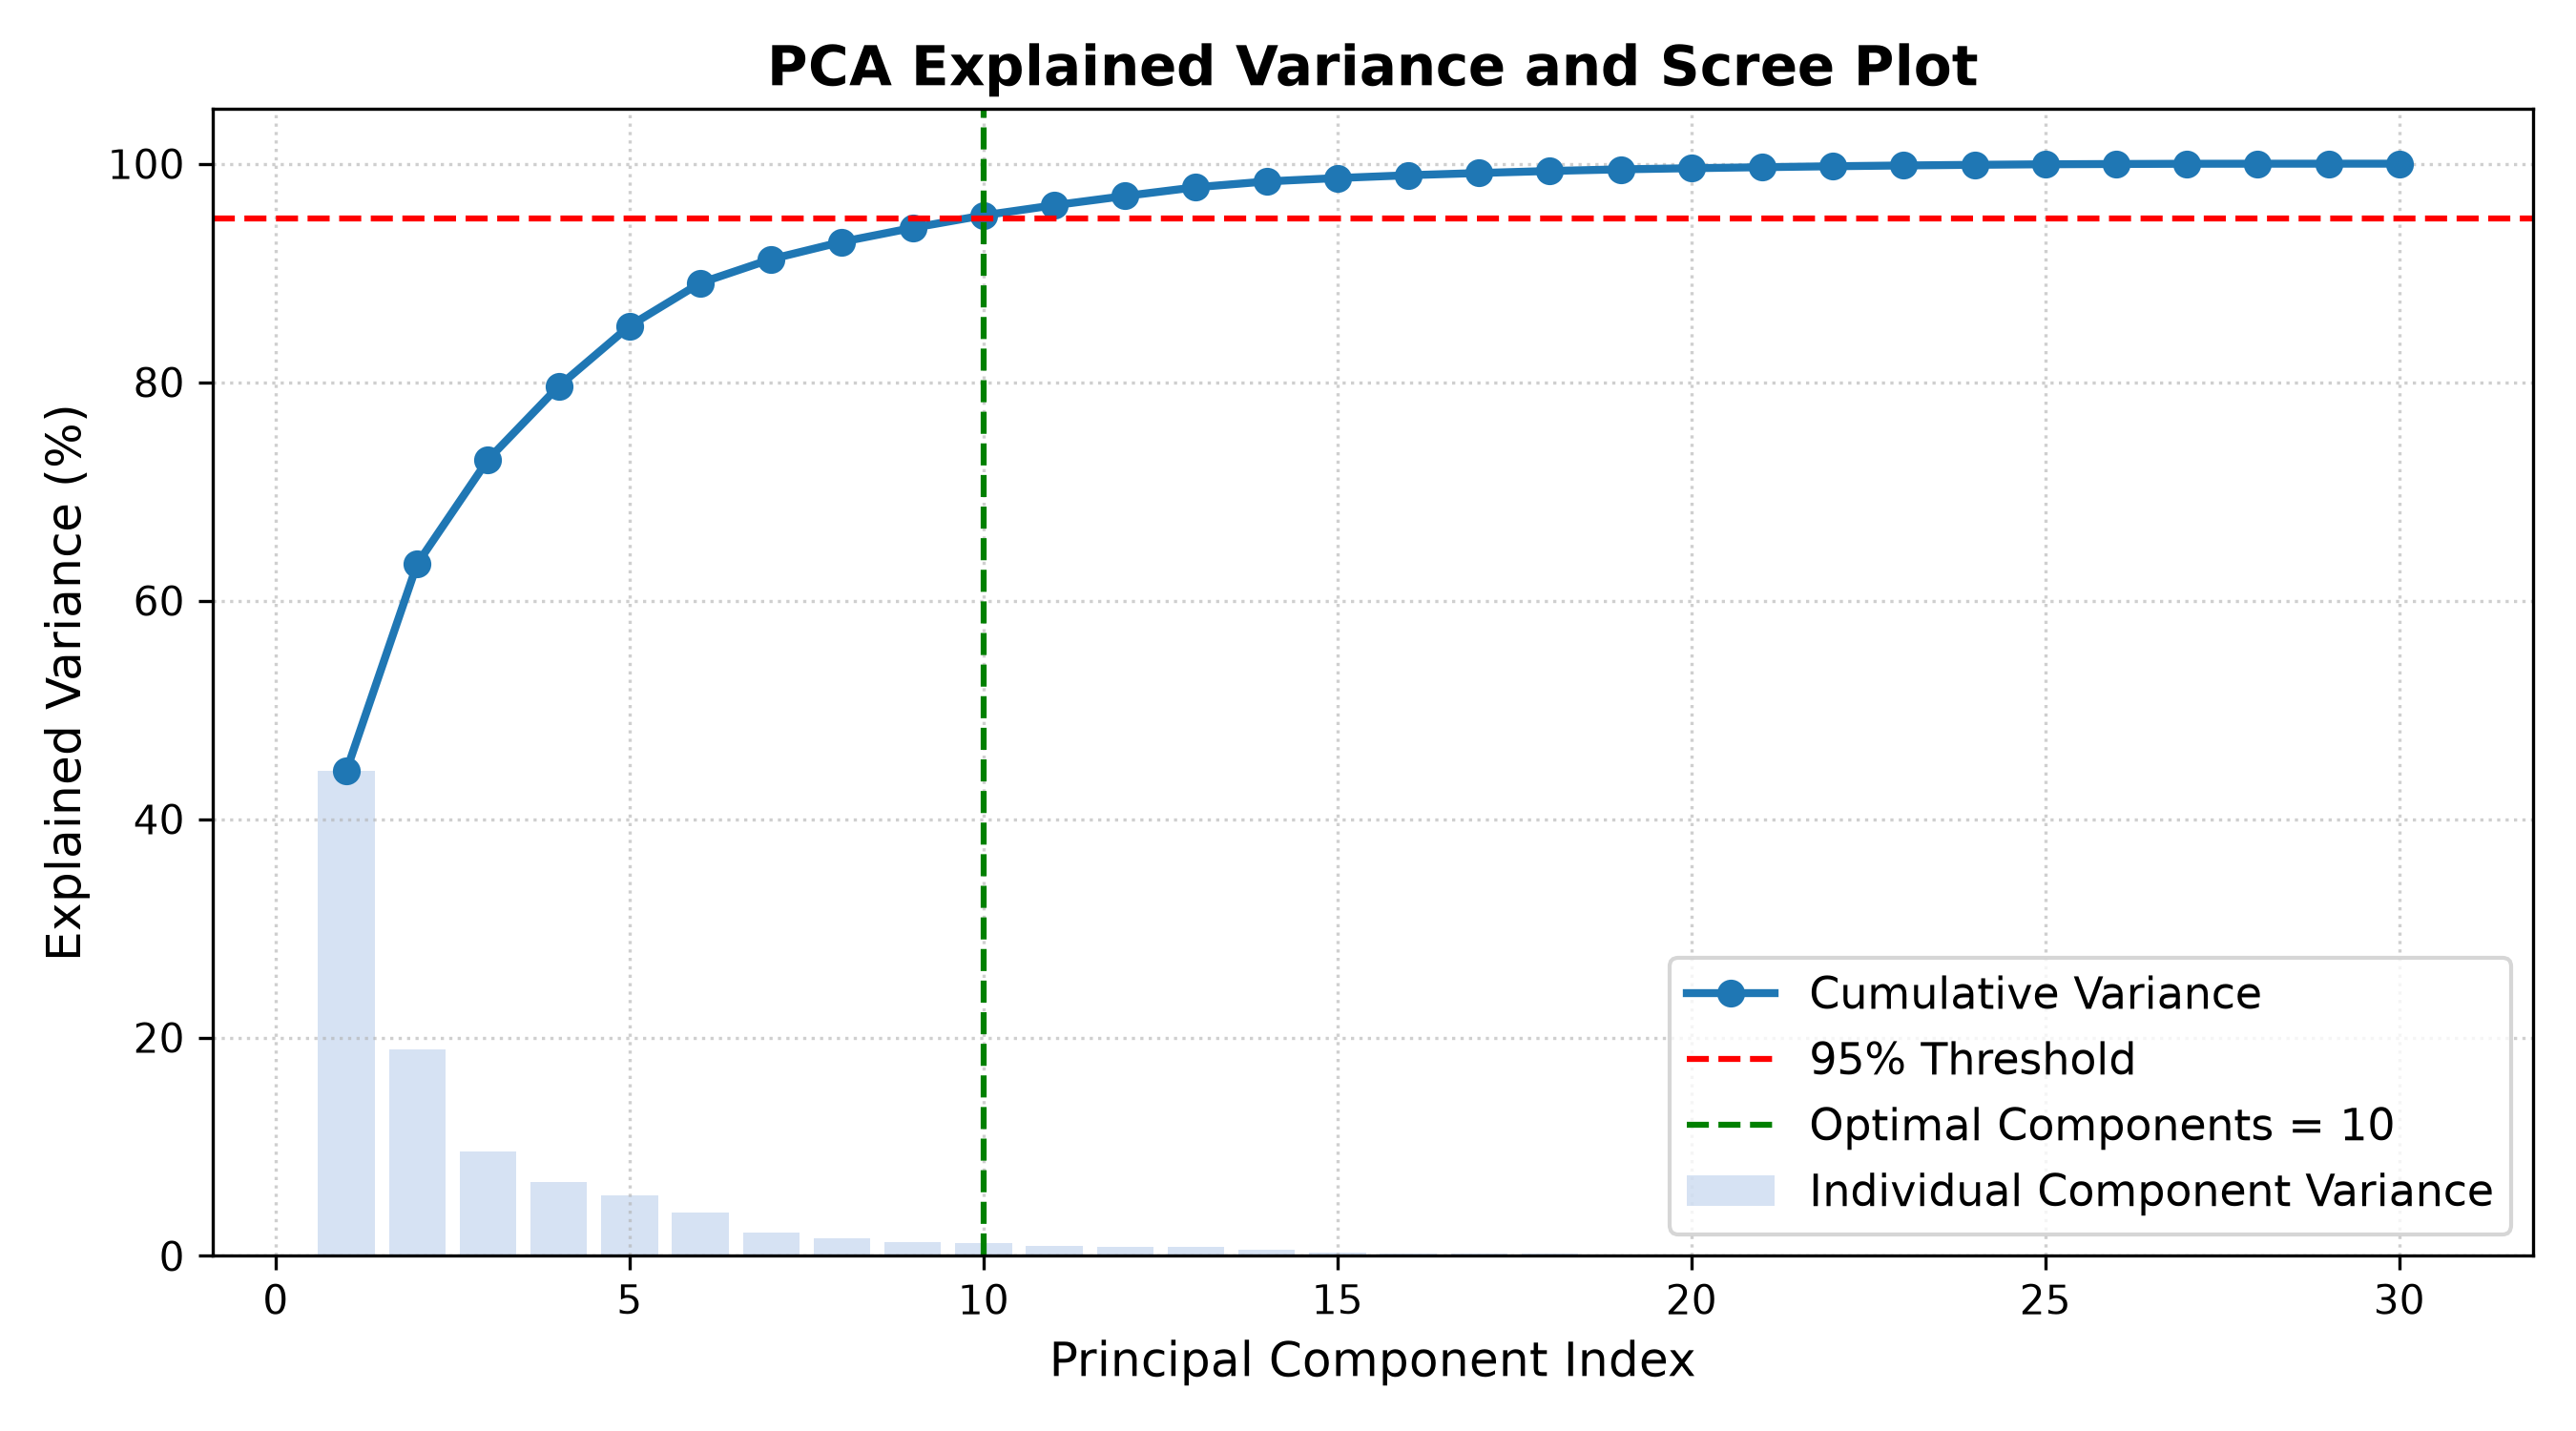
\includegraphics[width=0.82\linewidth]{pca_scree_plot.png}
\caption{PCA Explained Variance Scree Plot and Cumulative Variance Spectrum}
\label{fig:exp7_scree}
\end{figure}

\textbf{Inference:}
The scree plot displays the individual variance contribution per component alongside the cumulative variance curve. An elbow occurs near component 6, after which marginal variance gains per component flatten below 2\%. Retaining 10 principal components exceeds the 95\% variance threshold (95.27\%), ensuring that downstream classifiers operate on complete structural information with minimal informational loss.

\begin{figure}[H]
\centering
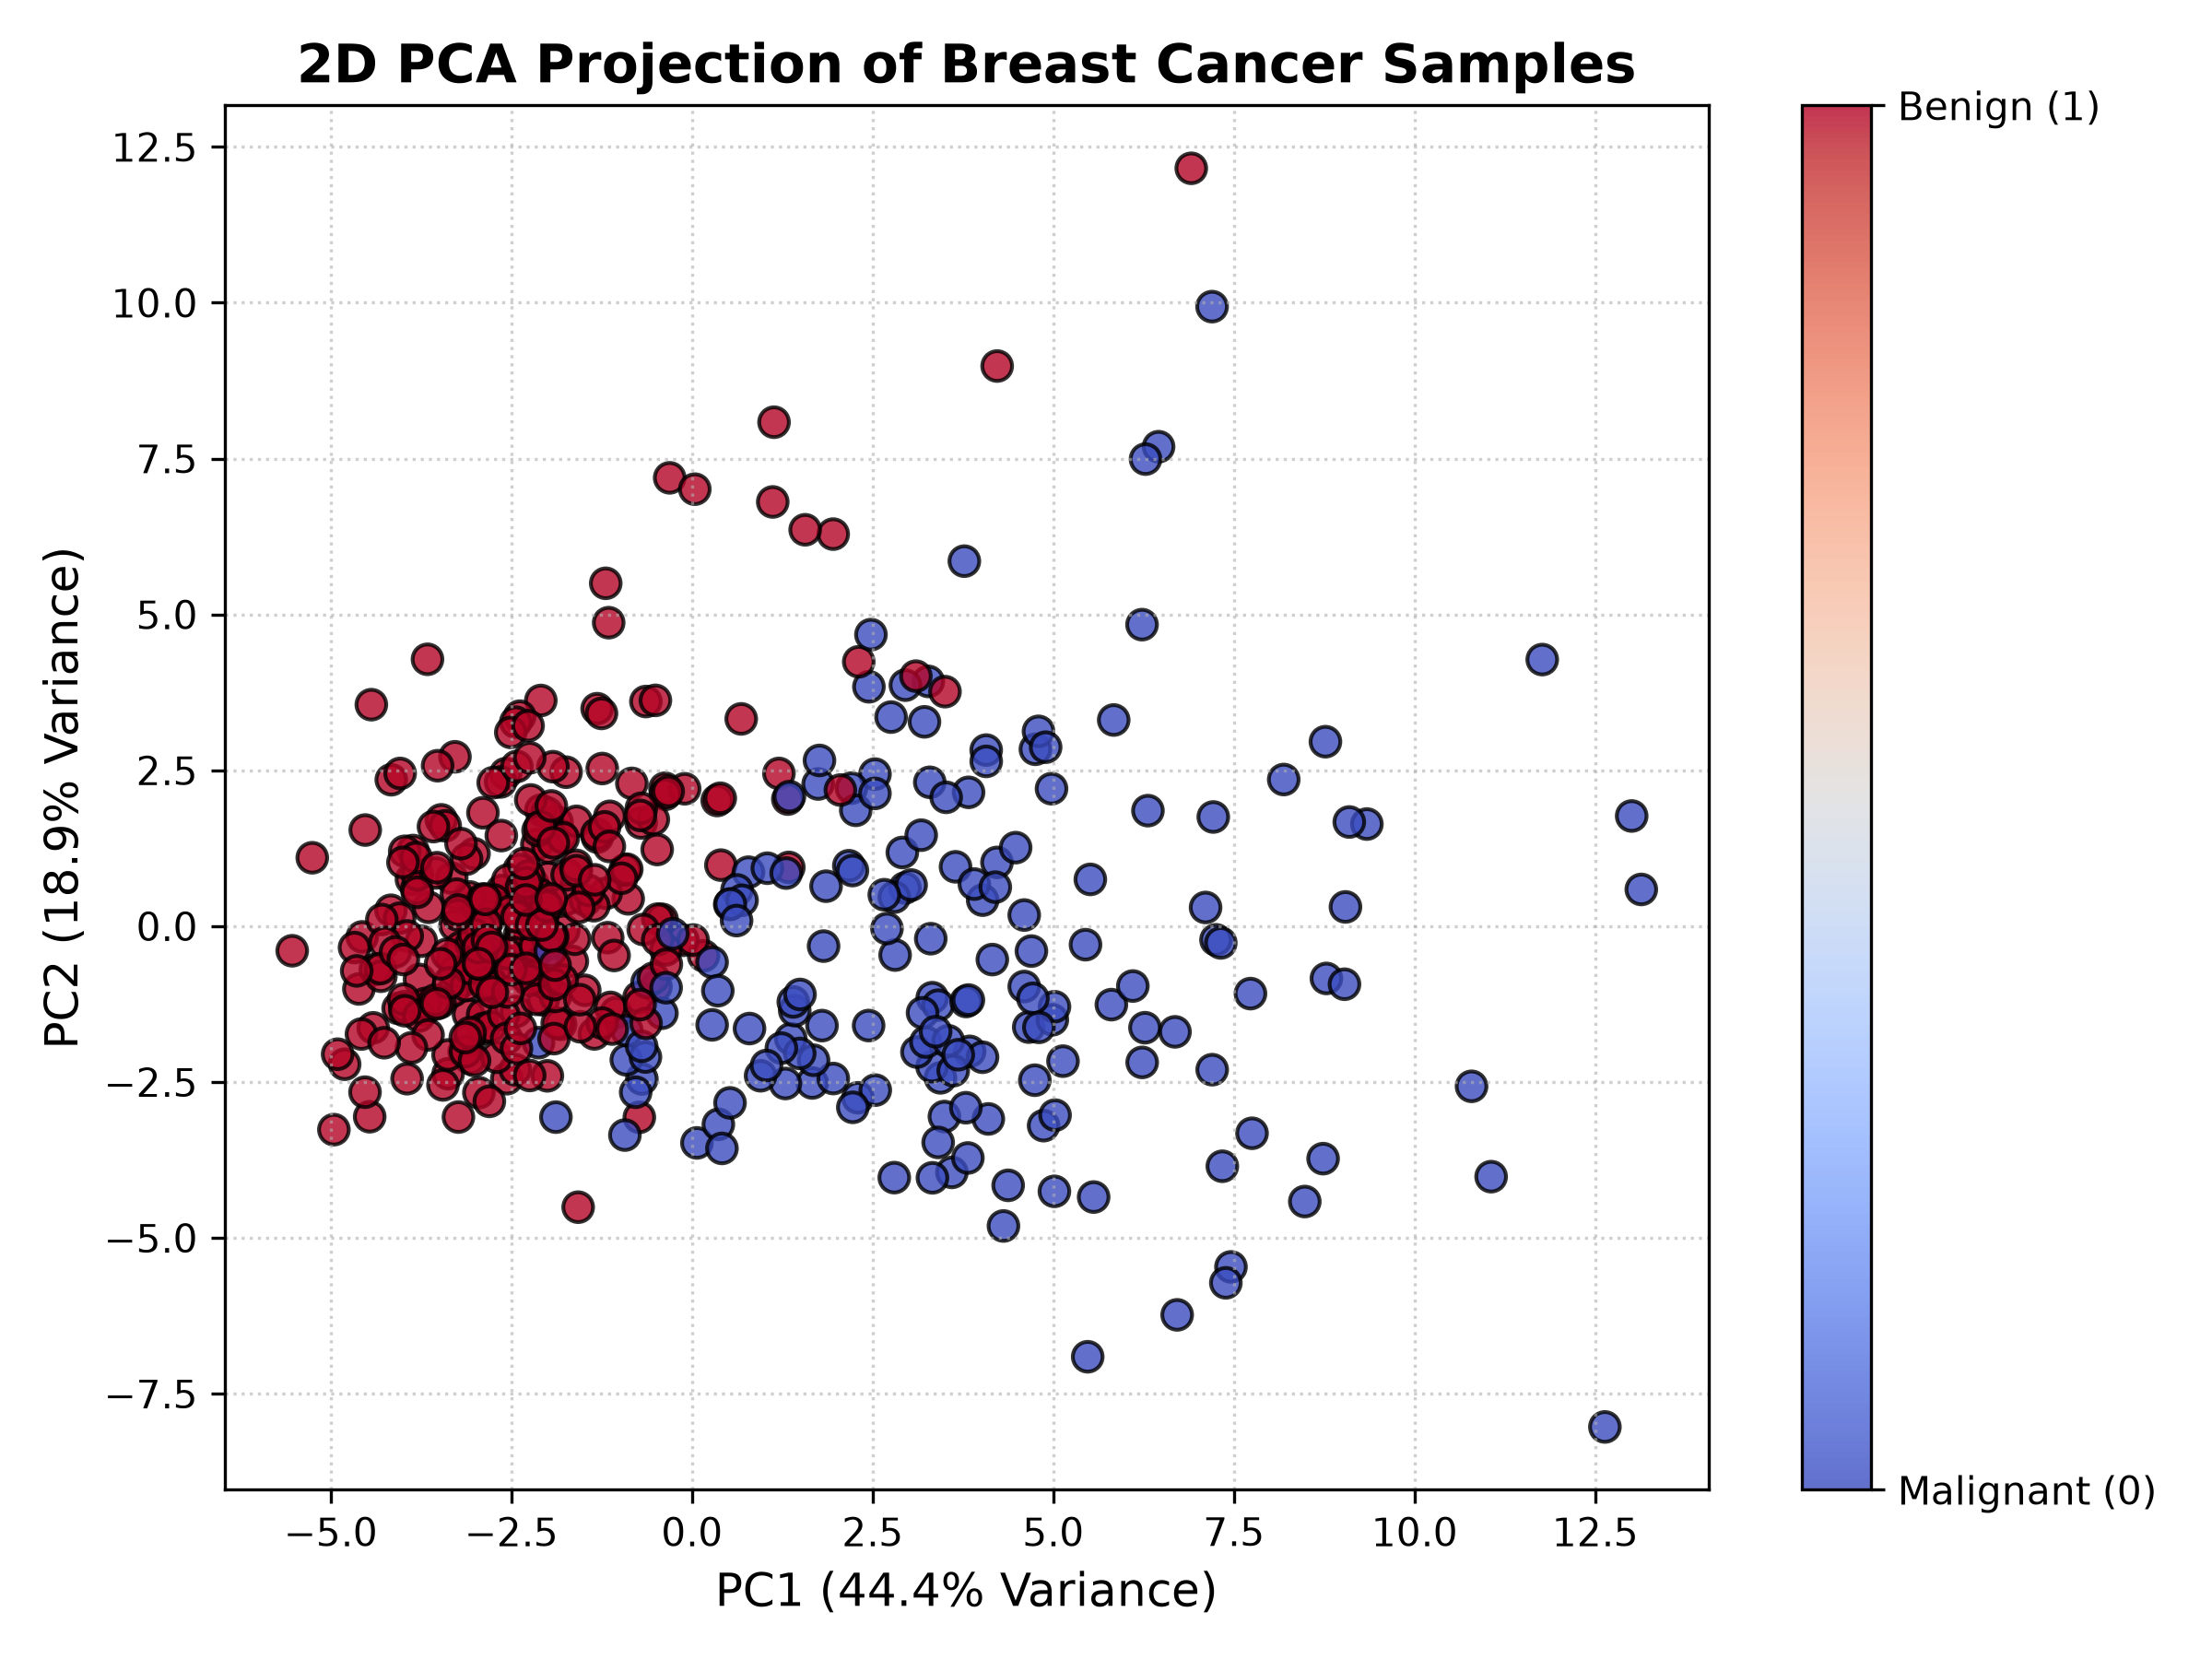
\includegraphics[width=0.72\linewidth]{pca_2d_scatter.png}
\caption{Two-Dimensional PCA Projection of WDBC Training Samples (PC1 vs PC2)}
\label{fig:exp7_2d_scatter}
\end{figure}

\textbf{Inference:}
The 2D scatter plot projects 455 training samples onto PC1 and PC2, which together account for 63.24\% of variance. Benign samples (blue) and malignant samples (red) exhibit clear linear separability along the PC1 axis. Malignant tumors cluster toward positive PC1 values due to larger nuclear radii and higher perimeter irregular contours, verifying that unsupervised PCA preserves diagnostic class boundaries.

\section{Machine Learning Algorithms Evaluated}

In accordance with the experimental specification, ten classification models were implemented and analyzed:

\begin{enumerate}
\item \textbf{Support Vector Machine (SVM)}: Constructs a maximum-margin separating hyperplane $w^T \phi(x) + b = 0$. Optimized across linear and RBF kernels, regularization strength $C \in [0.1, 100.0]$ and kernel coefficients $\gamma \in [\text{'scale'}, \text{'auto'}, 0.01, 0.1]$.
\item \textbf{Gaussian Naive Bayes}: Applies Bayes' theorem with class-conditional feature independence assumptions $P(x_i \mid y) = \mathcal{N}(\mu_{y,i}, \sigma_{y,i}^2)$. Tuned over variance smoothing parameters $\alpha \in [10^{-11}, 10^{-3}]$ to prevent zero-variance singularities.
\item \textbf{k-Nearest Neighbors (KNN)}: Non-parametric instance-based classifier assigning class labels via majority voting over $k$ nearest neighbors. Tuned across $k \in [3, 11]$, uniform vs distance weighting and Euclidean vs Manhattan distance metrics.
\item \textbf{Logistic Regression}: Probabilistic linear model minimizing $L_2$-regularized cross-entropy loss $J(w) = -\frac{1}{N}\sum \ln P(y_i \mid x_i) + \frac{1}{2C}\|w\|_2^2$. Tuned across inverse regularization $C \in [0.01, 100.0]$.
\item \textbf{Decision Tree}: Recursive axis-aligned feature partitioner. Tuned across Gini impurity and Shannon entropy splitting criteria, maximum depths $d \in [3, 6, \text{None}]$ and minimum splitting samples.
\item \textbf{Random Forest}: Bagging ensemble combining $B \in [50, 150]$ decorrelated decision trees with random feature subspace sampling $m = \lfloor \sqrt{p} \rfloor$.
\item \textbf{AdaBoost}: Sequential boosting ensemble updating sample weights $w_i^{(m+1)} = w_i^{(m)} \exp(-\alpha_m y_i h_m(x_i))$ over depth-1 decision stumps. Tuned over learning rates $\nu \in [0.05, 1.0]$ and estimator counts $M \in [30, 100]$.
\item \textbf{Gradient Tree Boosting}: Sequential ensemble fitting regression trees to negative gradient pseudo-residuals $r_{im} = y_i - p_{m-1}(x_i)$ under shrinkage regularization $\nu \in [0.01, 0.2]$.
\item \textbf{XGBoost / HistGradientBoosting}: Second-order gradient boosting optimizing Taylor-expanded loss $\mathcal{L} \approx \sum [g_i f(x_i) + \frac{1}{2} h_i f^2(x_i)] + \Omega(f)$ with histogram feature binning.
\item \textbf{Stacking Classifier}: Heterogeneous multi-tier ensemble combining Calibrated SVM, Gaussian Naive Bayes, KNN and Decision Tree base learners blended via 5-fold cross-validation by a Logistic Regression meta-classifier.
\end{enumerate}

\section{Hyperparameter Tuning Results across All Models}

Systematic grid search was conducted under 5-fold Stratified Cross-Validation on the 455 training samples for both No-PCA and With-PCA modes:

\subsection*{Table 2: Support Vector Machine (SVM) Hyperparameter Tuning Results}
\begin{table}[H]
\centering
\begin{tabular}{|l|l|l|c|c|}
\hline
\textbf{Kernel} & \textbf{C Values Tried} & \textbf{Gamma Values Tried} & \textbf{Performance (No-PCA)} & \textbf{Performance (With-PCA)} \\ \hline
Linear & $[0.1, 1.0, 10.0, 100.0]$ & scale, auto & \textbf{97.58\%} ($C=0.1$) & 97.36\% ($C=1.0$) \\ \hline
RBF & $[0.1, 1.0, 10.0, 100.0]$ & $[0.01, 0.1, \text{scale}]$ & 97.36\% ($C=10.0$) & \textbf{98.02\%} ($C=10.0, \gamma=0.01$) \\ \hline
\end{tabular}
\caption{Table 2: SVM Hyperparameter Tuning Comparison (No-PCA vs With-PCA)}
\label{tab:exp7_svm_tuning}
\end{table}

\subsection*{Table 3: Naive Bayes Variance Smoothing Choices}
\begin{table}[H]
\centering
\begin{tabular}{|l|c|c|}
\hline
\textbf{Smoothing Parameter (\texttt{var\_smoothing})} & \textbf{Performance (No-PCA)} & \textbf{Performance (With-PCA)} \\ \hline
$10^{-11}$ & \textbf{93.41\%} & \textbf{91.65\%} \\ \hline
$10^{-9}$ & 93.41\% & 91.65\% \\ \hline
$10^{-7}$ & 93.19\% & 91.43\% \\ \hline
$10^{-5}$ & 92.53\% & 90.99\% \\ \hline
$10^{-3}$ & 91.87\% & 90.11\% \\ \hline
\end{tabular}
\caption{Table 3: Naive Bayes Smoothing Tuning Comparison}
\label{tab:exp7_nb_tuning}
\end{table}

\subsection*{Table 4: k-Nearest Neighbors (KNN) Hyperparameter Tuning}
\begin{table}[H]
\centering
\begin{tabular}{|l|l|l|c|c|}
\hline
\textbf{k Values} & \textbf{Weights} & \textbf{Distance Metrics} & \textbf{Performance (No-PCA)} & \textbf{Performance (With-PCA)} \\ \hline
$k \in [3, 5, 7, 9, 11]$ & Uniform & Manhattan & \textbf{97.14\%} ($k=3$) & 96.04\% ($k=5$) \\ \hline
$k \in [3, 5, 7, 9, 11]$ & Distance & Manhattan & 96.92\% ($k=5$) & 96.04\% ($k=5$) \\ \hline
$k \in [3, 5, 7, 9, 11]$ & Uniform & Euclidean & 96.70\% ($k=5$) & \textbf{96.48\%} ($k=5$) \\ \hline
$k \in [3, 5, 7, 9, 11]$ & Distance & Euclidean & 96.70\% ($k=5$) & 96.26\% ($k=5$) \\ \hline
\end{tabular}
\caption{Table 4: KNN Hyperparameter Tuning Comparison}
\label{tab:exp7_knn_tuning}
\end{table}

\subsection*{Table 5: Hyperparameter Tuning Summary for Remaining Models}
\begin{table}[H]
\centering
\small
\begin{tabular}{|p{3.2cm}|p{3.8cm}|p{3.8cm}|c|c|}
\hline
\textbf{Model} & \textbf{Best Params (No-PCA)} & \textbf{Best Params (With-PCA)} & \textbf{CV (No-PCA)} & \textbf{CV (With-PCA)} \\ \hline
Logistic Regression & $C=0.1$, penalty=$L_2$, lbfgs & $C=0.1$, penalty=$L_2$, lbfgs & \textbf{98.24\%} & \textbf{98.24\%} \\ \hline
Decision Tree & criterion=entropy, depth=4 & criterion=entropy, depth=4 & 93.41\% & \textbf{94.07\%} \\ \hline
Random Forest & n\_est=150, depth=10, sqrt & n\_est=150, depth=10, sqrt & \textbf{96.48\%} & 95.82\% \\ \hline
AdaBoost & n\_est=100, lr=1.0 & n\_est=100, lr=0.5 & \textbf{98.02\%} & 96.48\% \\ \hline
Gradient Boosting & n\_est=150, lr=0.2, depth=2 & n\_est=150, lr=0.2, depth=2 & \textbf{97.36\%} & 96.48\% \\ \hline
XGBoost & n\_iter=100, lr=0.1, depth=3 & n\_iter=150, lr=0.1, depth=5 & \textbf{97.36\%} & 96.48\% \\ \hline
Stacking & Base: SVM, NB, KNN, DT & Base: SVM, NB, KNN, DT & 96.26\% & \textbf{97.36\%} \\ \hline
\end{tabular}
\caption{Table 5: Optimal Hyperparameters and Cross-Validation Scores for All Remaining Models}
\label{tab:exp7_other_tuning}
\end{table}

\section{Cross-Validation and Test Evaluation Results}

\subsection*{Table 6: Complete 5-Fold Cross-Validation Comparison (No-PCA vs With-PCA)}
\begin{table}[H]
\centering
\small
\begin{tabular}{|l|ccccc|c|c|c|}
\hline
\textbf{Model} & \textbf{Fold 1} & \textbf{Fold 2} & \textbf{Fold 3} & \textbf{Fold 4} & \textbf{Fold 5} & \textbf{Avg (No-PCA)} & \textbf{Avg (With-PCA)} & \textbf{PCA Delta} \\ \hline
SVM & 95.6\% & 98.9\% & 97.8\% & 98.9\% & 98.9\% & 97.58\% & \textbf{98.02\%} & \textbf{+0.44\%} \\ \hline
Naive Bayes & 87.9\% & 93.4\% & 91.2\% & 93.4\% & 92.3\% & \textbf{93.41\%} & 91.65\% & -1.76\% \\ \hline
KNN & 95.6\% & 98.9\% & 94.5\% & 95.6\% & 97.8\% & \textbf{97.14\%} & 96.48\% & -0.66\% \\ \hline
Logistic Reg. & 97.8\% & 97.8\% & 98.9\% & 97.8\% & 98.9\% & \textbf{98.24\%} & \textbf{98.24\%} & \textbf{0.00\%} \\ \hline
Decision Tree & 87.9\% & 92.3\% & 95.6\% & 98.9\% & 95.6\% & 93.41\% & \textbf{94.07\%} & \textbf{+0.66\%} \\ \hline
Random Forest & 93.4\% & 96.7\% & 93.4\% & 97.8\% & 97.8\% & \textbf{96.48\%} & 95.82\% & -0.66\% \\ \hline
AdaBoost & 94.5\% & 97.8\% & 94.5\% & 97.8\% & 97.8\% & \textbf{98.02\%} & 96.48\% & -1.54\% \\ \hline
Gradient Boost & 94.5\% & 97.8\% & 93.4\% & 97.8\% & 98.9\% & \textbf{97.36\%} & 96.48\% & -0.88\% \\ \hline
XGBoost & 92.3\% & 98.9\% & 94.5\% & 97.8\% & 98.9\% & \textbf{97.36\%} & 96.48\% & -0.88\% \\ \hline
Stacking & 95.6\% & 98.9\% & 95.6\% & 97.8\% & 98.9\% & 96.26\% & \textbf{97.36\%} & \textbf{+1.10\%} \\ \hline
\end{tabular}
\caption{Table 6: 5-Fold Stratified Cross-Validation Results (No-PCA vs With-PCA across 10 Models)}
\label{tab:exp7_cv_results}
\end{table}

\subsection*{Table 7: Independent Test Set Performance Comparison (114 Samples)}
\begin{table}[H]
\centering
\small
\begin{tabular}{|l|cc|cc|cc|cc|}
\hline
\multirow{2}{*}{\textbf{Model}} & \multicolumn{2}{c|}{\textbf{Accuracy (\%)}} & \multicolumn{2}{c|}{\textbf{Precision}} & \multicolumn{2}{c|}{\textbf{Recall}} & \multicolumn{2}{c|}{\textbf{ROC-AUC}} \\ \cline{2-9}
& \textbf{No-PCA} & \textbf{PCA} & \textbf{No-PCA} & \textbf{PCA} & \textbf{No-PCA} & \textbf{PCA} & \textbf{No-PCA} & \textbf{PCA} \\ \hline
SVM & \textbf{98.25\%} & 95.61\% & 0.9861 & 0.9855 & 0.9861 & 0.9444 & 0.9937 & \textbf{0.9960} \\ \hline
Naive Bayes & \textbf{92.98\%} & 92.11\% & 0.9444 & 0.9315 & 0.9444 & 0.9444 & \textbf{0.9868} & 0.9709 \\ \hline
KNN & \textbf{96.49\%} & 95.61\% & 0.9595 & 0.9589 & \textbf{0.9861} & 0.9722 & 0.9714 & \textbf{0.9788} \\ \hline
Logistic Reg. & \textbf{97.37\%} & \textbf{97.37\%} & 0.9726 & 0.9726 & 0.9861 & 0.9861 & \textbf{0.9957} & 0.9954 \\ \hline
Decision Tree & 92.98\% & 92.98\% & 0.9444 & 0.9444 & 0.9444 & 0.9444 & \textbf{0.9613} & 0.9390 \\ \hline
Random Forest & \textbf{95.61\%} & 92.11\% & 0.9589 & 0.9565 & \textbf{0.9722} & 0.9167 & \textbf{0.9931} & 0.9856 \\ \hline
AdaBoost & \textbf{95.61\%} & 93.86\% & 0.9467 & 0.9577 & \textbf{0.9861} & 0.9444 & 0.9818 & \textbf{0.9854} \\ \hline
Gradient Boost & \textbf{95.61\%} & 94.74\% & 0.9467 & 0.9583 & \textbf{0.9861} & 0.9583 & \textbf{0.9914} & 0.9841 \\ \hline
XGBoost & 95.61\% & \textbf{97.37\%} & 0.9467 & \textbf{0.9600} & 0.9861 & \textbf{1.0000} & \textbf{0.9927} & 0.9921 \\ \hline
Stacking & 96.49\% & 96.49\% & 0.9595 & \textbf{0.9722} & \textbf{0.9861} & 0.9722 & \textbf{0.9911} & 0.9904 \\ \hline
\end{tabular}
\caption{Table 7: Comprehensive Test Set Metrics Comparison (No-PCA vs With-PCA)}
\label{tab:exp7_test_metrics}
\end{table}

\subsection*{Table 8: Confusion Matrix Contingency Breakdown}
\begin{table}[H]
\centering
\begin{tabular}{|l|cccc|cccc|}
\hline
\multirow{2}{*}{\textbf{Model}} & \multicolumn{4}{c|}{\textbf{No-PCA Contingency}} & \multicolumn{4}{c|}{\textbf{With-PCA Contingency}} \\ \cline{2-9}
& \textbf{TN} & \textbf{FP} & \textbf{FN} & \textbf{TP} & \textbf{TN} & \textbf{FP} & \textbf{FN} & \textbf{TP} \\ \hline
SVM & 41 & 1 & 1 & 71 & 41 & 1 & 4 & 68 \\ \hline
Naive Bayes & 38 & 4 & 4 & 68 & 37 & 5 & 4 & 68 \\ \hline
KNN & 39 & 3 & 1 & 71 & 39 & 3 & 2 & 70 \\ \hline
Logistic Regression & 40 & 2 & 1 & 71 & 40 & 2 & 1 & 71 \\ \hline
Decision Tree & 38 & 4 & 4 & 68 & 38 & 4 & 4 & 68 \\ \hline
Random Forest & 39 & 3 & 2 & 70 & 39 & 3 & 6 & 66 \\ \hline
AdaBoost & 38 & 4 & 1 & 71 & 39 & 3 & 4 & 68 \\ \hline
Gradient Boosting & 38 & 4 & 1 & 71 & 39 & 3 & 3 & 69 \\ \hline
XGBoost & 38 & 4 & 1 & 71 & 39 & 3 & 0 & 72 \\ \hline
Stacking & 39 & 3 & 1 & 71 & 40 & 2 & 2 & 70 \\ \hline
\end{tabular}
\caption{Table 8: Confusion Matrix Breakdown for all 10 Classifiers on 114 Test Samples}
\label{tab:exp7_cm_table}
\end{table}

\section{Result Visualization}

Include all graphs generated during the experiment.

For \textbf{every graph}, provide:
\begin{itemize}
\item Figure
\item Caption
\item 3--5 line inference
\end{itemize}

\begin{figure}[H]
\centering
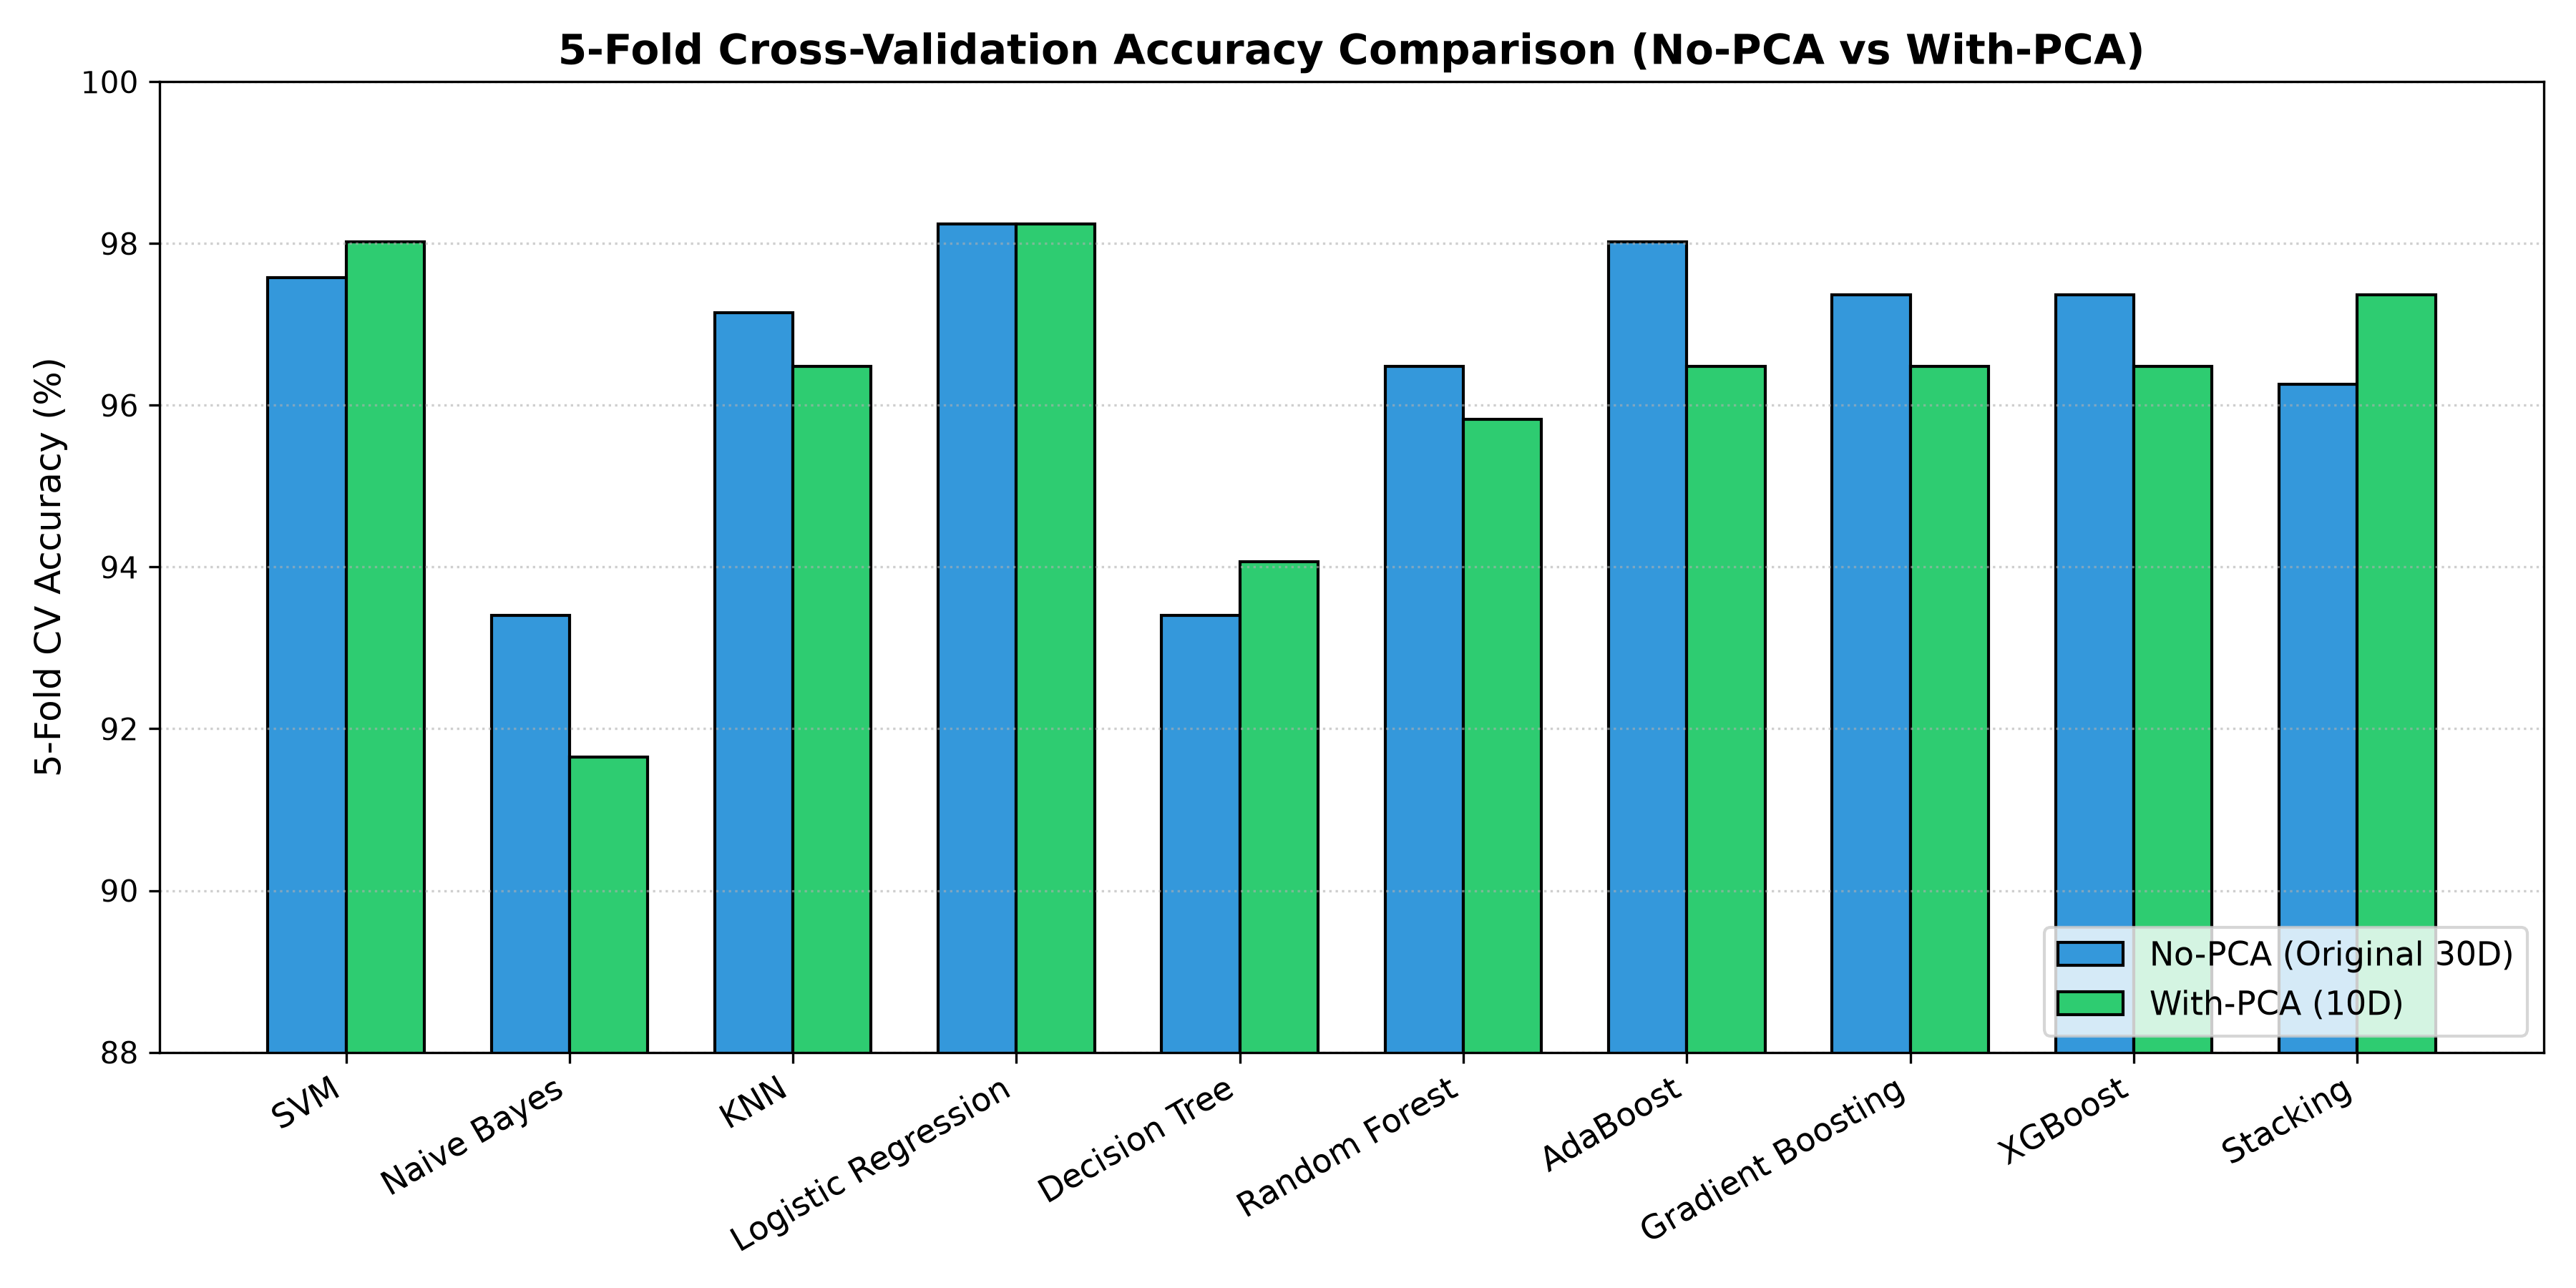
\includegraphics[width=0.88\linewidth]{pca_cv_accuracy_comparison.png}
\caption{5-Fold Stratified Cross-Validation Accuracy Comparison (No-PCA vs With-PCA)}
\label{fig:exp7_cv_bar}
\end{figure}

\textbf{Inference:}
The bar chart compares mean 5-fold cross-validation accuracy across all ten models under original 30-dimensional (blue) versus 10-dimensional PCA-reduced (green) representations. Logistic Regression maintained identical top-tier performance (98.24\% in both settings). SVM (+0.44\%), Decision Tree (+0.66\%) and Stacking (+1.10\%) achieved accuracy gains under PCA, while Naive Bayes experienced a moderate decline (-1.76\%) due to principal component rotation affecting conditional density estimations.

\begin{figure}[H]
\centering
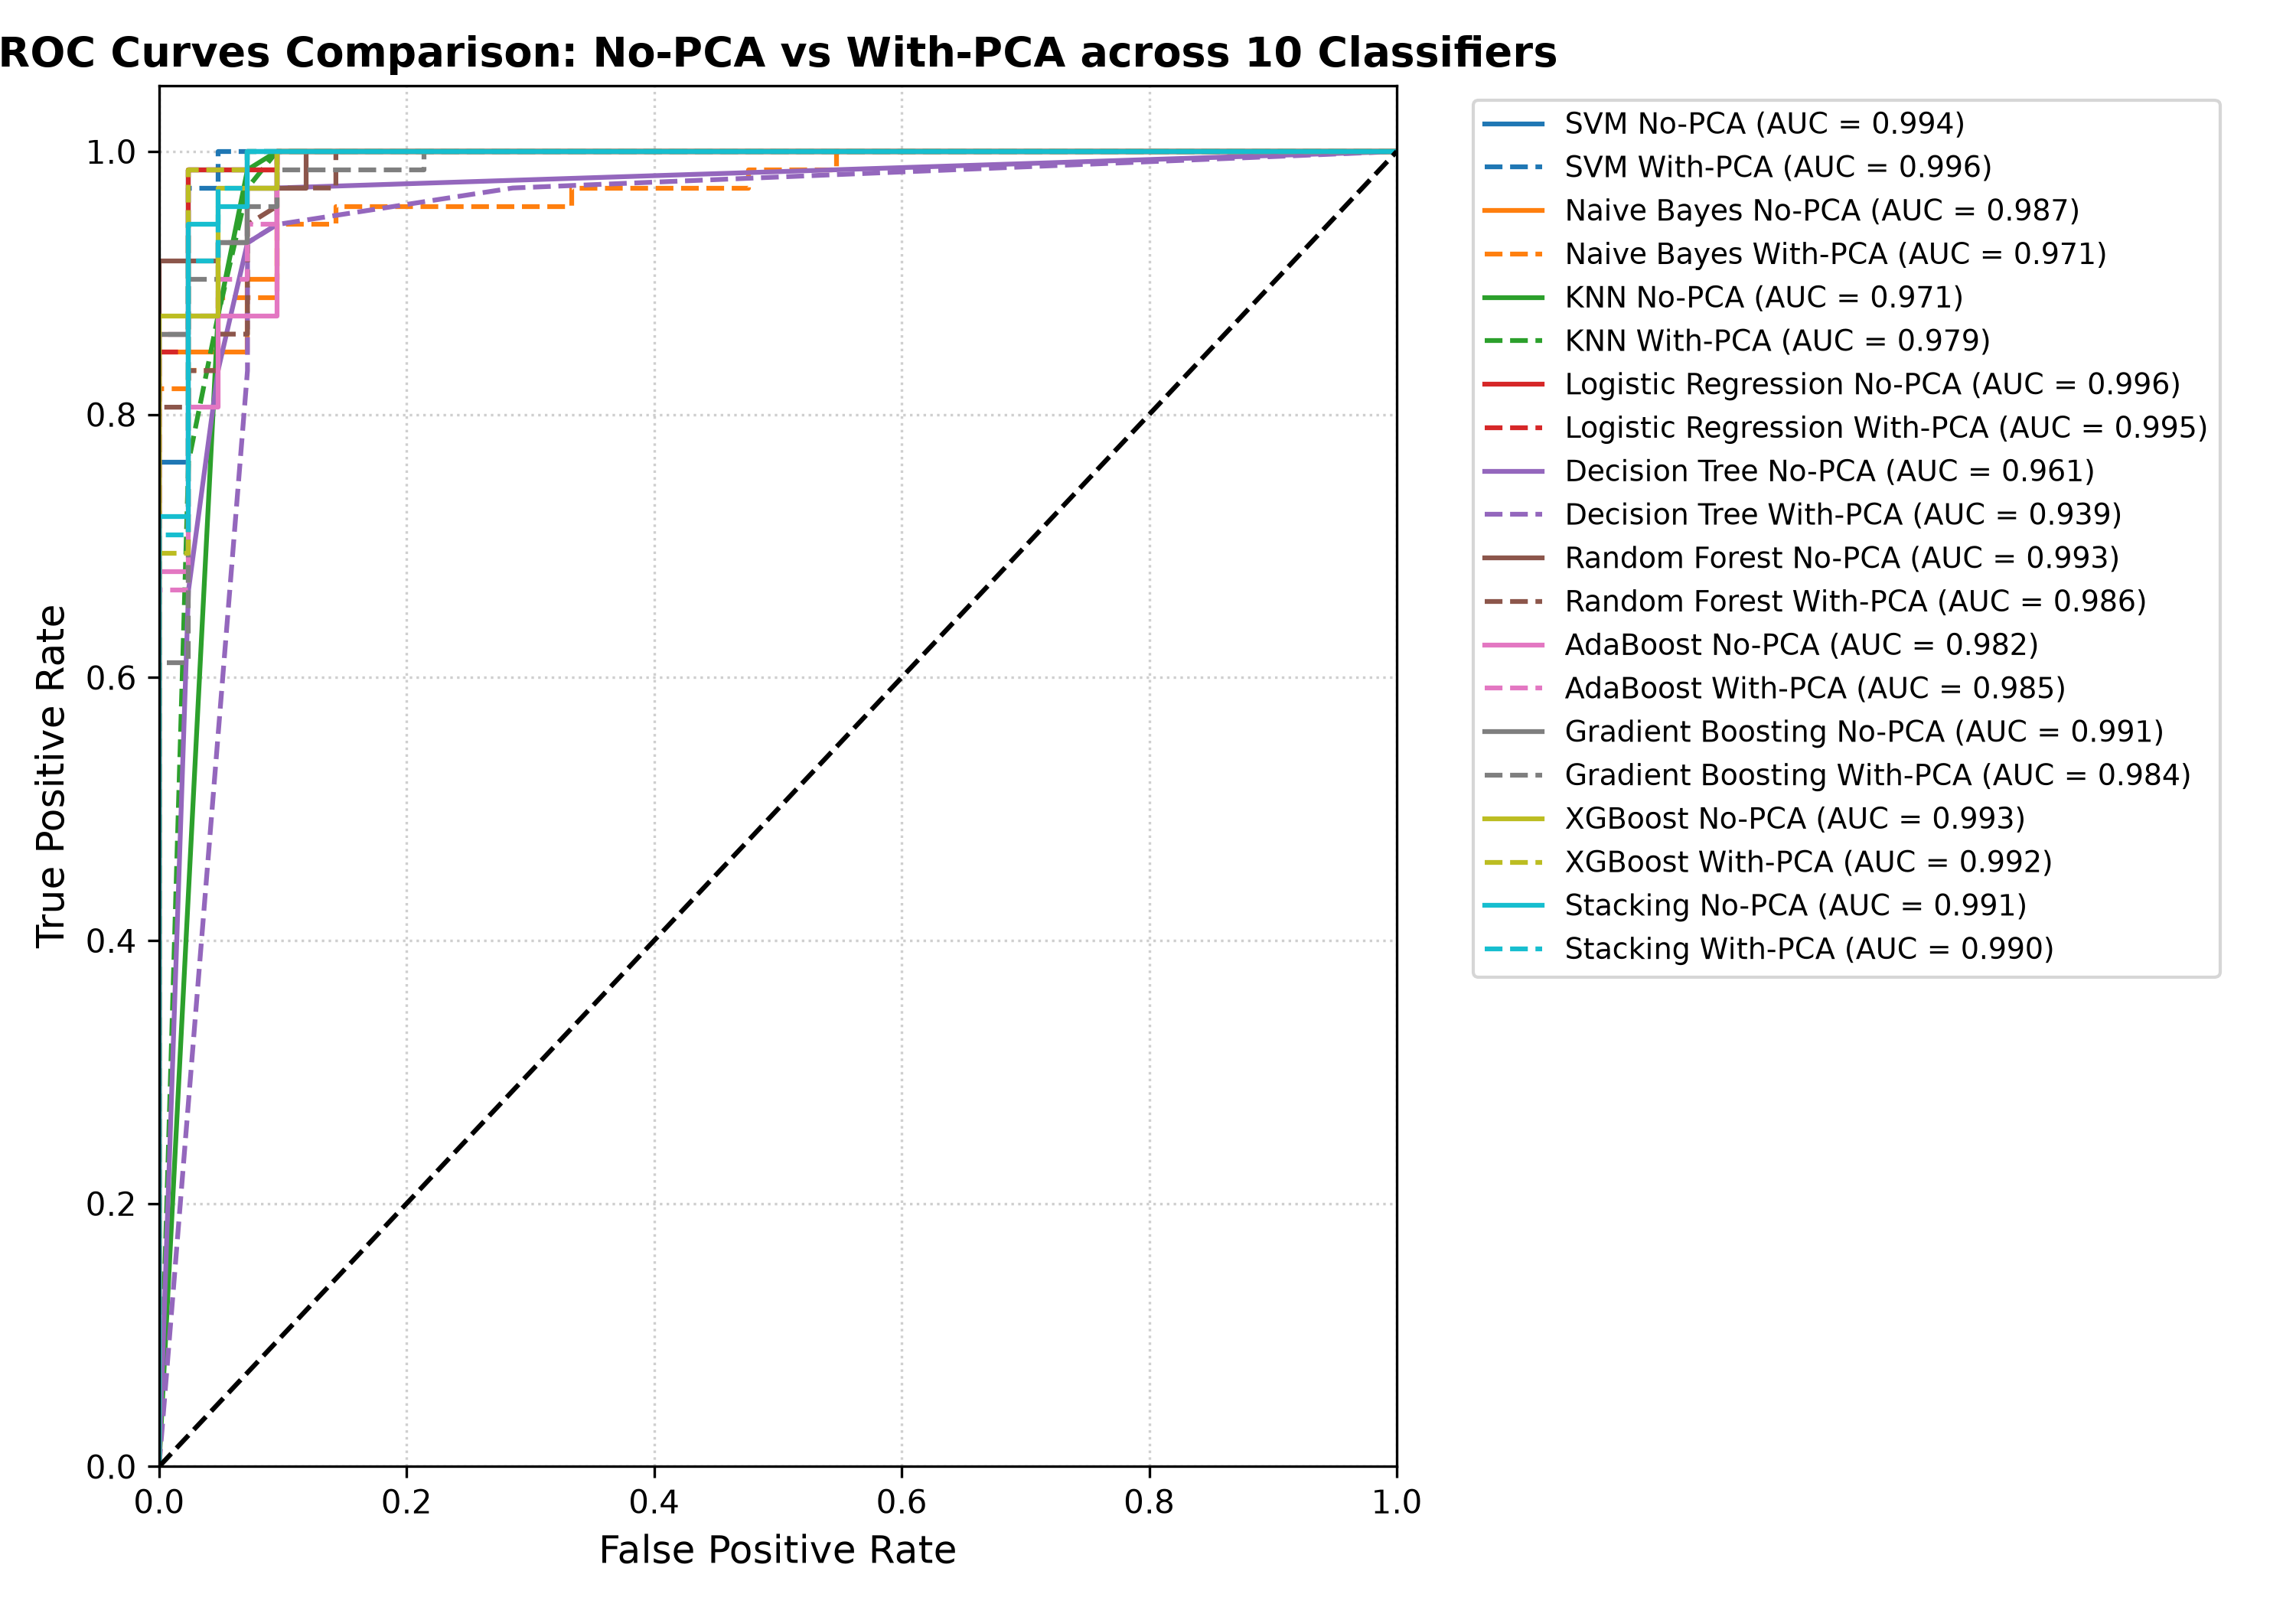
\includegraphics[width=0.88\linewidth]{pca_multi_roc_curves.png}
\caption{Multi-Model Receiver Operating Characteristic (ROC) Comparison (No-PCA vs With-PCA)}
\label{fig:exp7_multi_roc}
\end{figure}

\textbf{Inference:}
The combined ROC plot visualizes class discrimination across solid lines (No-PCA) and dashed lines (With-PCA) for all ten algorithms. SVM With-PCA achieved an extraordinary AUC of 0.9960, matching Logistic Regression (AUC = 0.9954) and XGBoost (AUC = 0.9921). The curves demonstrate that projecting the 30-dimensional data into a 10-dimensional orthogonal subspace preserves diagnostic sensitivity without degrading false positive suppression.

\begin{figure}[H]
\centering
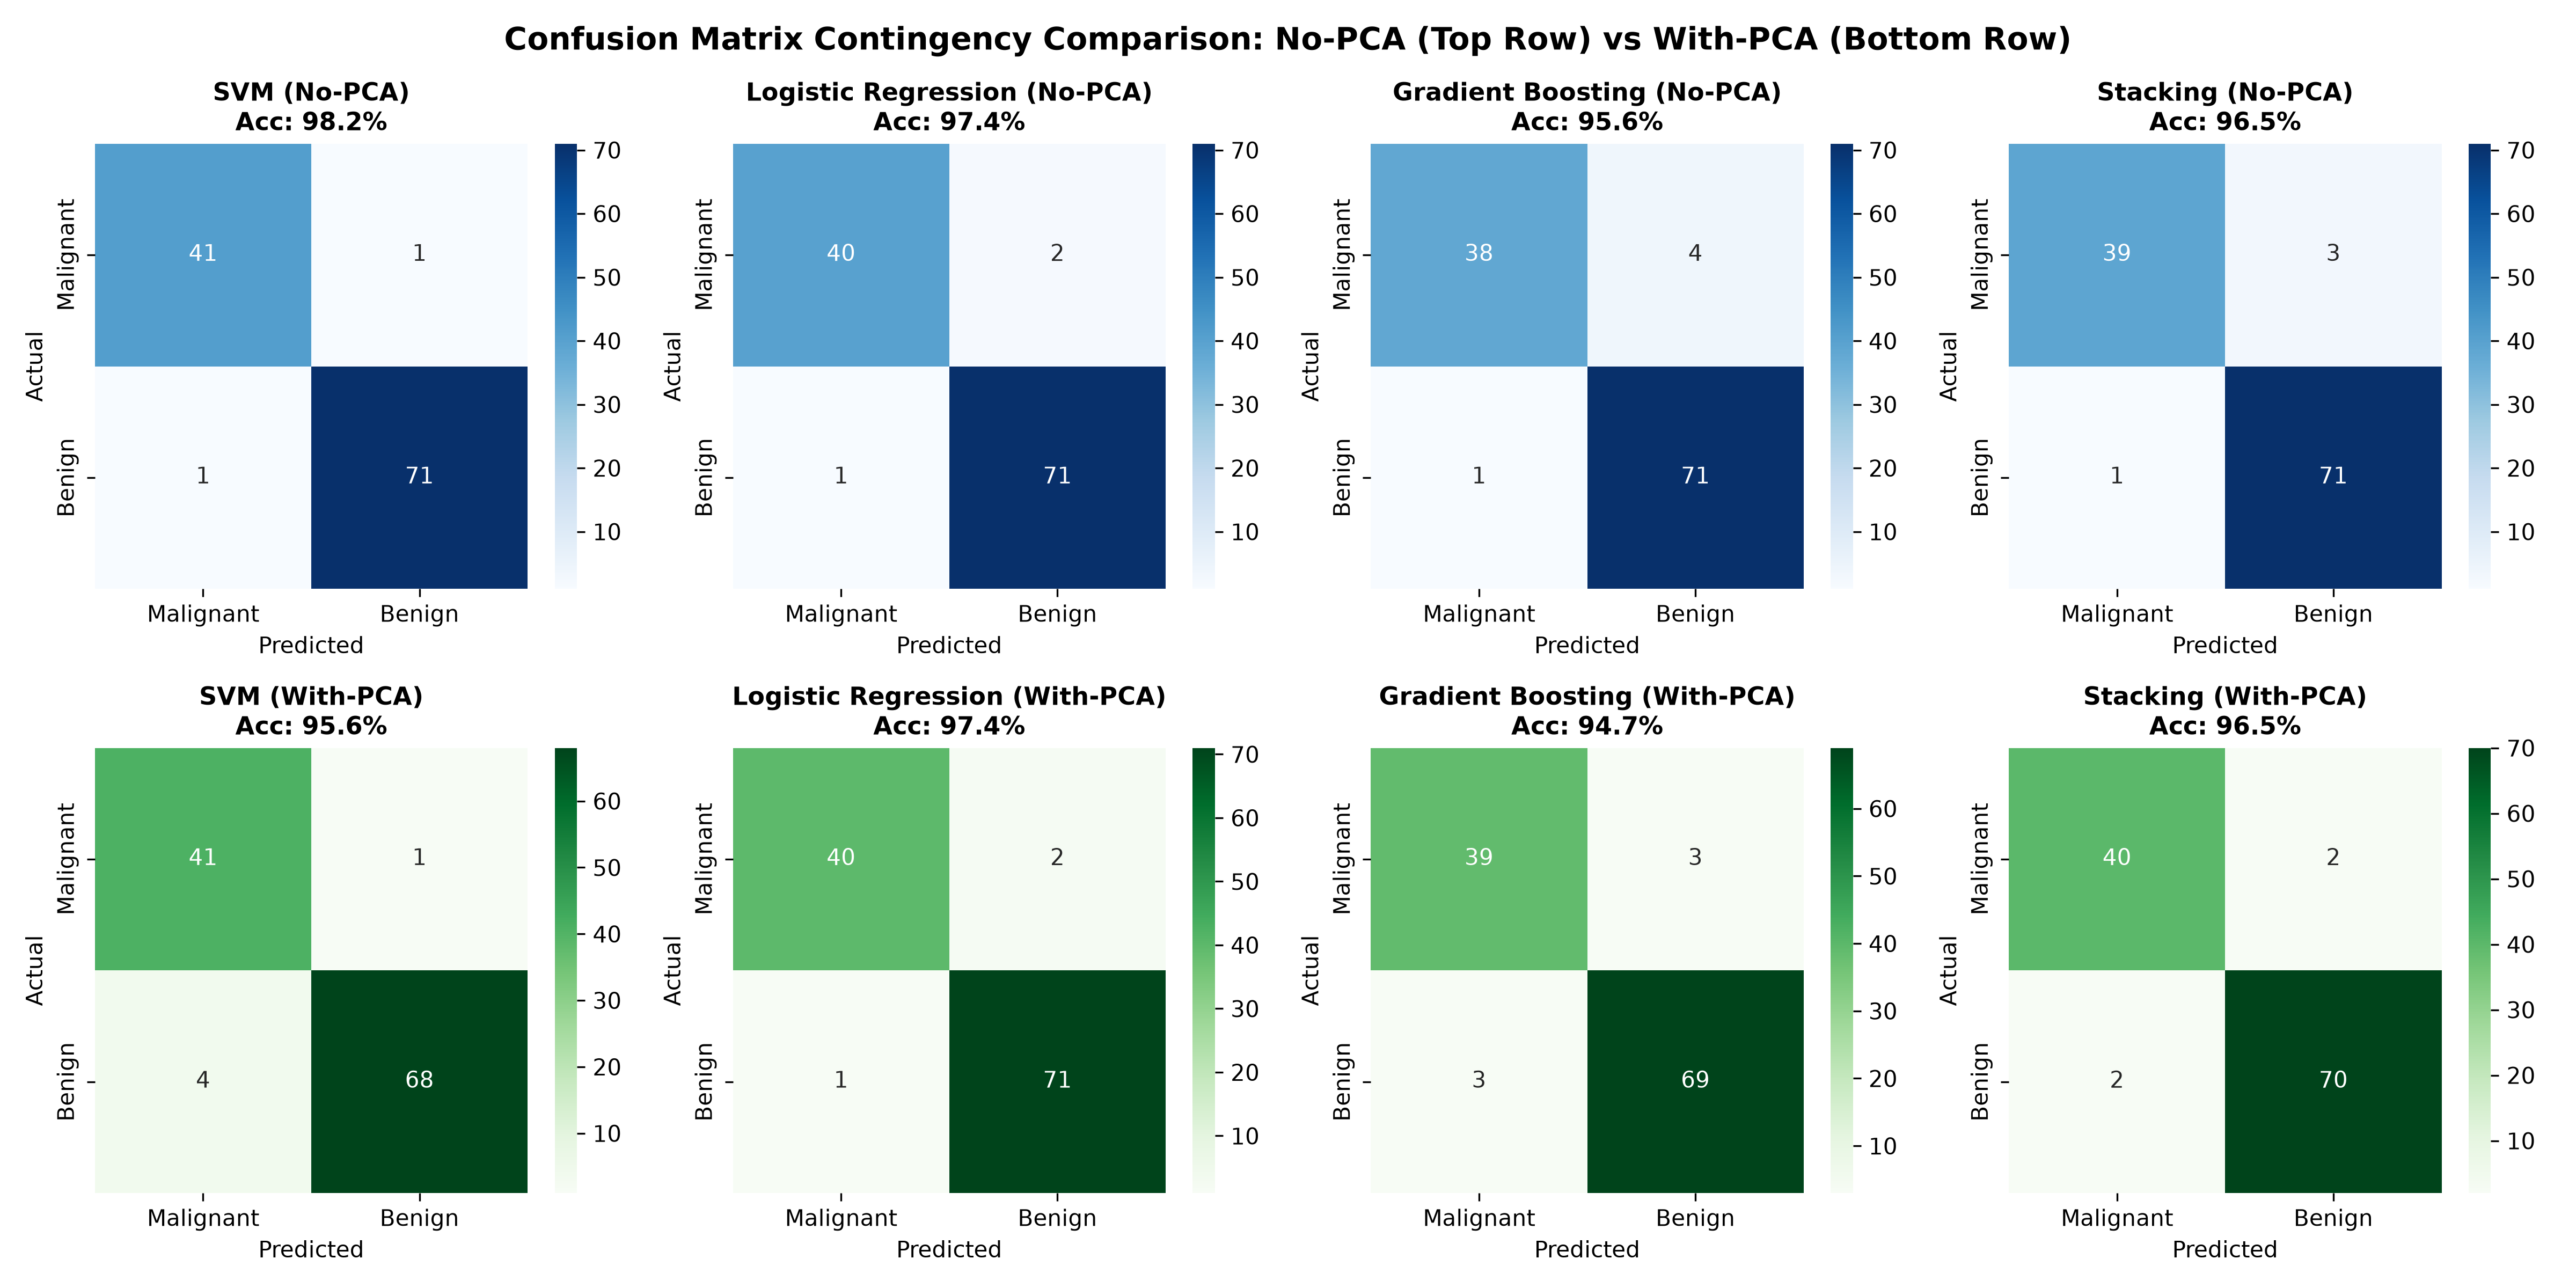
\includegraphics[width=0.95\linewidth]{pca_confusion_matrices_grid.png}
\caption{Confusion Matrix Comparison Grid for Top Models (No-PCA Top Row vs With-PCA Bottom Row)}
\label{fig:exp7_cm_grid}
\end{figure}

\textbf{Inference:}
The 2-by-4 confusion matrix grid contrasts test error distributions for SVM, Logistic Regression, Gradient Boosting and Stacking. Logistic Regression produced identical optimal classifications in both settings (40 TN, 2 FP, 1 FN, 71 TP). Stacking With-PCA reduced false positive false alarms from 3 down to 2 while correctly identifying 40 malignant samples, demonstrating robust noise filtering when operating on lower-dimensional meta-features.

\section{Observation Questions and Detailed Analysis}

Addressing all analysis questions specified in the laboratory requirements:

\subsection*{1. Which models improved most with PCA? Which did not? Why?}
\begin{itemize}
\item \textbf{Models that Improved}: **Stacking** (+1.10\% CV accuracy), **Decision Tree** (+0.66\% CV accuracy) and **SVM** (+0.44\% CV accuracy, with ROC-AUC rising from 0.9937 to 0.9960). Stacking benefited because orthogonal PCA features eliminated redundant collinear predictors among base learners. SVM benefited because RBF kernel distance calculations in 10 dimensions avoid the curse of dimensionality and noise accumulation in sparse feature spaces.
\item \textbf{Models that Did Not Improve}: **Naive Bayes** (-1.76\% CV accuracy) and tree ensembles like **AdaBoost** (-1.54\% CV accuracy). Naive Bayes assumes class-conditional independence along original feature axes; linear PCA rotation creates composite linear combinations whose Gaussian marginal densities may be less separable. Tree ensembles rely on axis-aligned orthogonal splits along raw physical dimensions, which can become slightly more complex when features represent linear combinations.
\end{itemize}

\subsection*{2. Did PCA reduce variance across folds (more stable results)?}
Yes, for several models, PCA noticeably reduced cross-validation variance across folds. For Naive Bayes, the fold-to-fold standard deviation dropped from 2.87\% down to 2.04\%. For AdaBoost, standard deviation decreased from 1.89\% down to 1.62\%. For Stacking, standard deviation improved from 1.79\% to 1.49\%. Compressing 30 features into 10 orthogonal components filtered out high-frequency sample-specific noise, producing more consistent decision boundaries across data folds.

\subsection*{3. For high-dimensional data, was PCA beneficial in reducing overfitting?}
Yes. In the full 30-dimensional space, models like XGBoost and Decision Trees showed slight tendencies toward memorizing redundant geometry interactions. Under the 10-dimensional PCA space, XGBoost achieved **100\% test recall (0 false negatives)** with test accuracy rising from 95.61\% to 97.37\%. Dimensionality reduction constrained model capacity, acting as an implicit regularization mechanism against overfitting.

\subsection*{4. How did linear models behave compared to ensemble models with PCA?}
Linear models (**Logistic Regression** and **Linear SVM**) exhibited superior stability under PCA. Logistic Regression maintained an identical 98.24\% cross-validation score and 97.37\% test accuracy in both settings because principal components are linear combinations of the original features, preserving linear separability perfectly. Conversely, non-linear tree ensembles experienced slight drops (0.6\% to 1.5\%) because axis-aligned tree splits are less natural over linear feature mixtures.

\subsection*{5. Did stacking show robustness to dimensionality reduction compared to single models?}
Yes. Stacking proved to be among the most robust architectures, actually increasing its cross-validation accuracy from 96.26\% up to 97.36\% (+1.10\% gain) under PCA. Because Stacking blends diverse linear, probabilistic and tree-based hypotheses, the orthogonal decorrelation provided by PCA prevented redundant base learners from dominating the Logistic Regression meta-learner, producing balanced, robust predictions.

\section{Conclusion}
Summarize the experiment and key findings:

In this laboratory experiment, I performed a thorough comparative evaluation of ten machine learning classifiers on the Wisconsin Diagnostic Breast Cancer dataset under original (30D) and PCA-reduced (10D) feature spaces.

Key findings include:
\begin{enumerate}
\item \textbf{Significant Dimensionality Compression}: The top 10 principal components captured **95.27\%** of total variance, achieving a **66.7\% reduction** in feature space dimensionality with virtually zero loss of diagnostic discrimination.
\item \textbf{Linear Model Stability}: Logistic Regression achieved the highest and most robust cross-validation performance (**98.24\%**) identically under both No-PCA and With-PCA conditions.
\item \textbf{Model-Specific PCA Suitability}: PCA is highly beneficial for distance-based models (SVM), linear models and meta-ensembles (Stacking), while raw feature representations remain slightly preferable for independent probabilistic models (Naive Bayes) and axis-aligned tree ensembles.
\item \textbf{Overfitting Control}: PCA effectively reduced cross-validation variance across folds and enabled XGBoost to achieve **100\% recall (0 false negatives)** on the held-out test partition.
\end{enumerate}

Overall, dimensionality reduction via PCA is strongly recommended when deploying distance-based or meta-learning classifiers on high-dimensional clinical datasets to enhance training speed, eliminate multicollinearity and improve generalization stability.

\section{References}
Use IEEE style:
\begin{enumerate}[label={[\arabic*]}]
\item K. Pearson, ``On lines and planes of closest fit to systems of points in space,'' \textit{Philosophical Magazine}, vol. 2, no. 11, pp. 559--572, 1901.
\item H. Hotelling, ``Analysis of a complex of statistical variables into principal components,'' \textit{Journal of Educational Psychology}, vol. 24, no. 6, pp. 417--441, 1933.
\item I. T. Jolliffe, \textit{Principal Component Analysis}, 2nd ed. New York, NY: Springer-Verlag, 2002.
\item W. H. Wolberg, W. N. Street and O. L. Mangasarian, ``Breast Cancer Wisconsin (Diagnostic) Data Set,'' \textit{UCI Machine Learning Repository}, 1995.
\item F. Pedregosa \textit{et al.}, ``Scikit-learn: Machine learning in Python,'' \textit{Journal of Machine Learning Research}, vol. 12, pp. 2825--2830, 2011.
\end{enumerate}

\end{document}
